\documentclass{../../../oss-apphys}
\usepackage{bm}

\begin{document}
\genheader

\gentitle{1}{KINEMATICS}

\genmultidirections

\gengravity

\raggedcolumns
\begin{multicols}{2}

  \textbf{Questions 1--2}

  A ball of mass \SI{.5}{\kilo\gram} is launched horizontally from the top of a
  cliff \SI{80}{\metre} high with a speed of \SI{20}{\metre\per\second} at time
  $t=0$.
  \begin{center}
    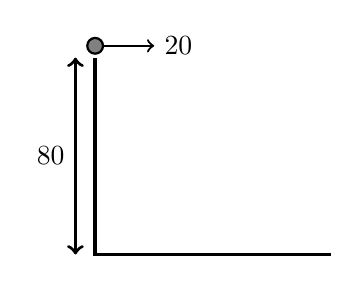
\begin{tikzpicture}[scale=.5]
      \draw[very thick](0,5)--(0,0)--(6,0);
      \draw[<->,very thick](-.5,0)--(-.5,5) node[midway,left]{\SI{80}{\metre}};
      \draw[thick,->](0,5.3)--(1.5,5.3)
      node[pos=1,right]{\SI{20}{\metre\per\second}};
      \draw[thick,fill=gray](0,5.3) circle(.2);
    \end{tikzpicture}
  \end{center}
  \begin{enumerate}[leftmargin=18pt]
  \item The horizontal distance $x$ traveled by the ball before striking the
    ground is
    \begin{enumerate}[nosep,leftmargin=18pt,label=(\Alph*)]
    \item\SI{20}{\metre}
    \item\SI{40}{\metre}
    \item\SI{80}{\metre} 
    \item\SI{160}{\metre}
    \item\SI{320}{\metre}
    \end{enumerate}

  \item The speed of the ball just before striking the ground is
    \begin{enumerate}[nosep,leftmargin=18pt,label=(\Alph*)]
    \item\SI{4}{\metre\per\second}
    \item\SI{14}{\metre\per\second}
    \item\SI{20}{\metre\per\second}
    \item\SI{44}{\metre\per\second}
    \item\SI{64}{\metre\per\second}
    \end{enumerate}

  \item A space explorer throws a tool downward on a planet with an initial
    velocity of \SI{2}{\metre\per\second} from a height of \SI{6}{\metre}
    above the surface. The
    tool strikes the surface in a time of \SI{2}{\second}. The acceleration due
    to gravity on the planet is
    \begin{enumerate}[nosep,leftmargin=18pt,label=(\Alph*)]
    \item\SI{1}{\metre\per\second\squared}
    \item\SI{2}{\metre\per\second\squared}
    \item\SI{3}{\metre\per\second\squared}
    \item\SI{4}{\metre\per\second\squared}
    \item\SI{10}{\metre\per\second\squared}
    \end{enumerate}
  \end{enumerate}
  \columnbreak

  \textbf{Questions \ref{q:sprinter1}--\ref{q:sprinter2}}
  
  A sprinter starting from rest runs a \SI{100}{\metre} race on a straight
  track. The sprinter covers the first \SI{10}{\metre} with a constant
  acceleration in 2 seconds. The sprinter runs the remaining \SI{90}{\metre}
  with the same velocity he had at the end of \SI{2}{\second}.

  \begin{enumerate}[resume,leftmargin=18pt]
  \item The sprinter's velocity at the end of the first \SI{2}{\second} is
    \begin{enumerate}[nosep,leftmargin=18pt,label=(\Alph*)]
    \item\SI{5 }{\metre\per\second}
    \item\SI{10}{\metre\per\second}
    \item\SI{20}{\metre\per\second}
    \item\SI{40}{\metre\per\second}
    \item\SI{60}{\metre\per\second}
    \end{enumerate}
    \label{q:sprinter1}

  \item The total time it takes for the sprinter to run the full
    \SI{100}{\metre} is
    \begin{enumerate}[nosep,leftmargin=18pt,label=(\Alph*)]
    \item\SI{2 }{\second}
    \item\SI{9 }{\second}
    \item\SI{10}{\second}
    \item\SI{11}{\second}
    \item\SI{12}{\second}
    \end{enumerate}
    \label{q:sprinter2}
    
  \item A block of mass \SI{2}{\kilo\gram} is attached to a string that is
    wrapped around a pulley of negligible mass and allowed to descend from rest
    a vertical distance of \SI{1.2}{\metre} in a time of \SI{1.5}{\second}. The
    acceleration of the block is most nearly
    \vspace{-.2in}
    \cpic{.18}{block-pulley.png}
    \begin{enumerate}[nosep,leftmargin=18pt,label=(\Alph*)]
    \item\SI{0.2}{\metre\per\second\squared}
    \item\SI{.6} {\metre\per\second\squared}
    \item\SI{1.1}{\metre\per\second\squared}
    \item\SI{1.4}{\metre\per\second\squared}
    \item\SI{1.5}{\metre\per\second\squared}
    \end{enumerate}

  \item A ball is attached to a string of length \SI{.8}{\metre} and is swung
    in a vertical circle. The bottom of the circle is \SI{.2}{\metre} above the
    floor. If the string breaks at the top of the circle when the speed of the
    ball is \SI{5}{\metre\per\second}, the horizontal distance the ball travels
    before striking the floor is
    \vspace{-.2in}
    \cpic{.15}{ball-string.png}
    \begin{enumerate}[nosep,leftmargin=18pt,label=(\Alph*)]
    \item\SI{.8 }{\metre}
    \item\SI{2.3 }{\metre}
    \item\SI{3.0 }{\metre}
    \item\SI{5.0 }{\metre}
    \item\SI{13.2}{\metre}
    \end{enumerate}
    
  \item A golf ball is hit from level ground and has a horizontal range of
    \SI{100}{\metre}. The ball leaves the golf club at an angle of \ang{60} to
    the level ground. At what other angle(s) can the ball be struck at the same
    initial velocity and still have a range of \SI{100}{\metre}?
    \begin{center}
      \vspace{-.2in}
      \pic{.25}{golf-ball.png}
    \end{center}
    \begin{enumerate}[nosep,leftmargin=18pt,label=(\Alph*)]
    \item\ang{30}
    \item\ang{20} and \ang{80}
    \item\ang{10} and \ang{120}
    \item\ang{45} and \ang{135}
    \item There is no other angle other than \ang{60} in which the ball will
      have a range of \SI{100}{\metre}.
    \end{enumerate}
    
  \item A small airplane can fly at \SI{200}{\kilo\metre\per\hour} with no
    wind. The pilot of the plane would like to fly to a destination
    \SI{100}{\kilo\metre} due north of his present position, but there is a
    crosswind of \SI{50}{\kilo\metre\per\hour} east. How much time is required
    for the plane to fly north to its destination?
    \begin{enumerate}[nosep,leftmargin=18pt,label=(\Alph*)]
    \item less than \SI{1/2}{\hour}
    \item \SI{1/2}{\hour}
    \item more than \SI{1/2}{\hour}
    \item \SI{1}{\hour}
    \item more than \SI{1}{\hour}
    \end{enumerate}
    
  \end{enumerate}
  \columnbreak
  
  \textbf{Questions \ref{q:particle1}--\ref{q:particle2}}

  A particle moves on a horizontal surface with a constant acceleration of
  \SI{6}{\metre\per\second\squared} in the $x$-direction and
  \SI{4}{\metre\per\second\squared} in the $y$-direction. The initial velocity
  of the particle is \SI{3}{\metre\per\second} in the $x$-direction.
  \begin{enumerate}[resume,leftmargin=18pt]
  \item The speed of the particle after \SI{4}{\second} is
    \begin{enumerate}[nosep,leftmargin=18pt,label=(\Alph*)]
    \item\SI{16}{\metre\per\second}
    \item\SI{27}{\metre\per\second}
    \item\SI{31}{\metre\per\second}
    \item\SI{44}{\metre\per\second}
    \item\SI{985}{\metre\per\second}
    \end{enumerate}
    \label{q:particle1}
    
  \item The displacement of the particle from its initial position is
    \begin{enumerate}[nosep,leftmargin=18pt,label=(\Alph*)]
    \item\SI{16}{\metre}
    \item\SI{32}{\metre}
    \item\SI{60}{\metre}
    \item\SI{68}{\metre}
    \item\SI{92}{\metre}
    \end{enumerate}
    \label{q:particle2}
    
  \item A small ball is launched with a speed of \SI{8}{\metre\per\second} at
    an angle of \ang{30} from the horizontal. A cup is hung so that it is in
    position to catch the ball when it reaches its maximum height. How far
    above the floor should the cup be hung to catch the ball?
    \cpic{.32}{cup.png}
    \begin{enumerate}[nosep,leftmargin=18pt,label=(\Alph*)]
    \item\SI{2.4}{\metre}
    \item\SI{1.6}{\metre}
    \item\SI{1.}{\metre}
    \item\SI{.8}{\metre}
    \item\SI{.4}{\metre}
    \end{enumerate}
  \end{enumerate}
  \newpage
  
  \textbf{Questions \ref{q:graph1}--\ref{q:graph2}}

  The graph shown below represents the velocity vs.\ time graphs for two cars,
  $P$ and $Q$. Car $P$ begins with a speed $v_P$, and Car $Q$ begins with a
  speed $v_Q$ which is twice the velocity of Car $P$, that is, $v_Q=2v_P$.
  \begin{center}
    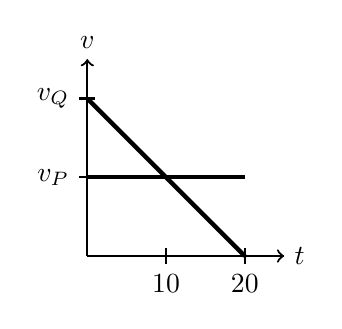
\begin{tikzpicture}[scale=.5]
      \draw[thick,->](0,0)--(5,0) node[pos=1,right]{$t$};
      \draw[thick,->](0,0)--(0,5) node[pos=1,above]{$v$};
      \draw[ultra thick](0,4)--(4,0);
      \draw[ultra thick](0,2)--(4,2);
      \draw[thick](2,.2)--(2,-.2) node[pos=1,below]{10};
      \draw[thick](4,.2)--(4,-.2) node[pos=1,below]{20};
      \draw[thick](.2,4)--(-.2,4) node[pos=1,left]{$v_Q$};
      \draw[thick](.2,2)--(-.2,2) node[pos=1,left]{$v_P$};
      \end{tikzpicture}
  \end{center}
  \begin{enumerate}[resume,leftmargin=18pt]
  \item Which of the following is true at a time of \SI{10}{\second}?
    \begin{enumerate}[nosep,leftmargin=18pt,label=(\Alph*)]
    \item The cars occupy the same position.
    \item Car $P$ is at rest.
    \item $v_Q>v_P$
    \item $v_P>v_Q$
    \item Car $Q$ is ahead of Car $P$.
    \end{enumerate}
    \label{q:graph1}
    \vspace{.65in}
    
  \item Which of the following is true at a time of \SI{20}{\second}?
    \begin{enumerate}[nosep,leftmargin=18pt,label=(\Alph*)]
    \item The cars occupy the same position.
    \item Car $P$ is at rest.
    \item $v_Q>v_P$
    \item $a_P=a_Q$
    \item Car $P$ is ahead of Car $Q$.
    \end{enumerate}
    \label{q:graph2}
    \vspace{.65in}
    
  \item The velocity vs.\ time graph below represents the motion of a bicycle
    rider. The displacement of the rider between $0$ and \SI{4}{\hour} is
    \cpic{.25}{bikerider}
    
    \begin{enumerate}[nosep,leftmargin=18pt,label=(\Alph*)]
    \item +\SI{10}{\kilo\metre}
    \item +\SI{20}{\kilo\metre}
    \item +\SI{30}{\kilo\metre}
    \item +\SI{40}{\kilo\metre}
    \item -\SI{10}{\kilo\metre}
    \end{enumerate}
    \columnbreak
    
  \item A car is initially moving with a positive velocity of
    \SI{20}{\metre\per\second} when it passes the origin at time $t=0$. The car
    continues to move at \SI{20}{\metre\per\second} between $t=0$ and
    $t=\SI{2}{\second}$. At $t=\SI{2}{\second}$, the driver presses the brake,
    giving the car an acceleration of \SI{-4}{\metre\per\second\squared}. The
    displacement of the car at $t=\SI{6}{\second}$ is
    \begin{enumerate}[nosep,leftmargin=18pt,label=(\Alph*)]
    \item\SI{40}{\metre}
    \item\SI{32}{\metre}
    \item\SI{48}{\metre}
    \item\SI{64}{\metre}
    \item\SI{88}{\metre}
    \end{enumerate}

  \item A ball is dropped from rest from the top of a cliff $80$ meters high. At
    the same time, a rock is thrown horizontally from the top of the same
    cliff. The rock and ball hit the level ground below a distance of
    \SI{40}{\metre} apart. The horizontal velocity of the rock that was thrown
    was most nearly
    \begin{center}
      \vspace{-.15in}\pic{.25}{ball-cliff.png}
    \end{center}
    \begin{enumerate}[nosep,leftmargin=18pt,label=(\Alph*)]
    \item\SI{5}{\metre\per\second}
    \item\SI{10}{\metre\per\second}
    \item\SI{20}{\metre\per\second}
    \item\SI{40}{\metre\per\second}
    \item\SI{80}{\metre\per\second}
    \end{enumerate}

  \item A \SI{600}{\kilo\gram} car accelerates uniformly from rest. After
    \SI{4}{\second}, it reaches a speed of \SI{24}{\metre\per\second}. During
    the \SI{4}{\second}, the car has traveled a distance of
    \begin{enumerate}[nosep,leftmargin=18pt,label=(\Alph*)]
    \item\SI{12}{\metre}
    \item\SI{24}{\metre}
    \item\SI{36}{\metre}
    \item\SI{48}{\metre}
    \item\SI{96}{\metre}
    \end{enumerate}
    \columnbreak
    
  \item Which of the following pairs of graphs could show the position vs.\
    time and velocity vs.\ time graphs for the acceleration vs. time graph
    shown above? Assume $v=0$ and $x=0$ at $t=0$.
    \begin{center}
      \begin{tikzpicture}[scale=.5]
        \draw[thick,->](0,0)--(8,0) node[pos=1,right]{$t$};
        \draw[thick,->](0,-3)--(0,3) node[pos=1,above]{$a$};
        \draw[ultra thick](0,2)--(2,2);
        \draw[ultra thick](2,0)--(4,0);
        \draw[ultra thick](4,-2)--(6,-2);
        \draw[ultra thick](6,0)--(8,0);
        \draw[thick,dashed](2,2)--(2,0);
        \draw[thick,dashed](4,0)--(4,-2);
        \draw[thick,dashed](6,0)--(6,-2);
      \end{tikzpicture}
    \end{center}
    \pic{.48}{xt-vt.png}
    \columnbreak
    
  \item Two velocity vectors $v_1$ and $v_2$ each have a magnitude of 10 m/s.
    Graph 1 shows the velocity $v_1$ at $t =\SI{0}{\second}$, and then the same
    object has a velocity $v_2$ at $t=\SI{2}{\second}$, shown in Graph 2. Which
    of the following vectors best represents the average acceleration vector
    that causes the object's velocity to change from $v_1$ to $v_2$ ?
    \begin{center}
      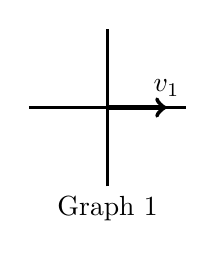
\begin{tikzpicture}[scale=.5]
        \draw[thick](-2,0)--(2,0);
        \draw[thick](0,-2)--(0,2) node[pos=0,below]{Graph 1};
        \draw[ultra thick,->](0,0)--(1.5,0) node[pos=1,above]{$v_1$};
      \end{tikzpicture}
      \hspace{.2in}
      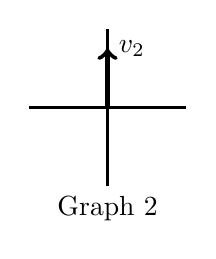
\begin{tikzpicture}[scale=.5]
        \draw[thick](-2,0)--(2,0);
        \draw[thick](0,-2)--(0,2) node[pos=0,below]{Graph 2};
        \draw[ultra thick,->](0,0)--(0,1.5) node[pos=1,right]{$v_2$};
      \end{tikzpicture}
    \end{center}
    \begin{enumerate}[nosep,leftmargin=18pt,label=(\Alph*)]
    \item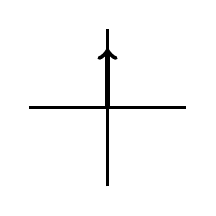
\begin{tikzpicture}[scale=.5]
      \draw[thick](-2,0)--(2,0);
      \draw[thick](0,-2)--(0,2);
        \draw[ultra thick,->](0,0)--(0,1.5);
    \end{tikzpicture}
    \item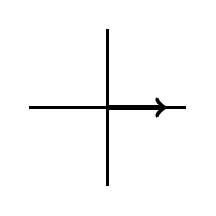
\begin{tikzpicture}[scale=.5]
      \draw[thick](-2,0)--(2,0);
      \draw[thick](0,-2)--(0,2);
      \draw[ultra thick,->](0,0)--(1.5,0);
    \end{tikzpicture}
    \item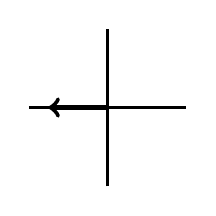
\begin{tikzpicture}[scale=.5]
        \draw[thick](-2,0)--(2,0);
        \draw[thick](0,-2)--(0,2);
        \draw[ultra thick,->](0,0)--(-1.5,0);
    \end{tikzpicture}
    \item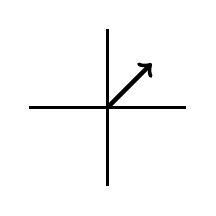
\begin{tikzpicture}[scale=.5]
      \draw[thick](-2,0)--(2,0);
      \draw[thick](0,-2)--(0,2);
        \draw[ultra thick,->](0,0)--(1.12,1.12);
    \end{tikzpicture}
    \item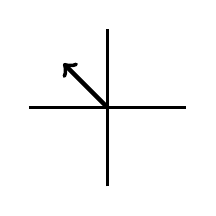
\begin{tikzpicture}[scale=.5]
      \draw[thick](-2,0)--(2,0);
      \draw[thick](0,-2)--(0,2);
        \draw[ultra thick,->](0,0)--(-1.12,1.12);
    \end{tikzpicture}
    \end{enumerate}
    \columnbreak

  \item A toy dart gun fires a dart at an angle of \ang{45} to the
    horizontal and the dart reaches a maximum height of 1 meter. If the dart
    were fired straight up into the air along the vertical, the dart would
    reach a height of
    \begin{enumerate}[nosep,leftmargin=18pt,label=(\Alph*)]
    \item\SI{1}{\metre}
    \item\SI{2}{\metre}
    \item\SI{3}{\metre}
    \item\SI{4}{\metre}
    \item\SI{5}{\metre}
    \end{enumerate}

  \item A ball is hit straight up into the air with an upward positive
    velocity. Wich of the following describes the velocity and acceleration
    of the ball at the instant it reaches the top of its flight?

    \begin{tabular}{lcc}
      & Velocity & Acceleration\\ \hline
      (A) & $0$ & $0$\\
      (B) & $0$ & $g$\\
      (C) & $2v_0$ & $g$\\
      (D) & $\displaystyle\frac12v_0$ & $0$\\
      (E) & $0$ & $\displaystyle\frac12g$
    \end{tabular}    
    \vspace{.65in}

  \item The motion of an object is represented by the acceleration vs.\ time
    graph below. The object begins from rest. Which of the following statements
    is true about the motion of the object?
    \begin{center}
      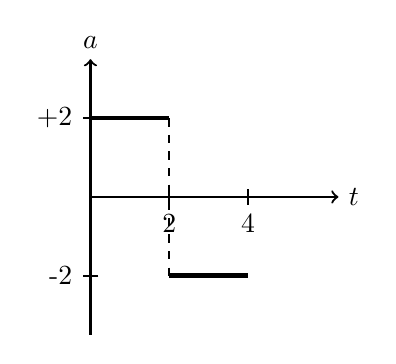
\begin{tikzpicture}[scale=.5]
        \draw[thick,->](0,0)--(6.3,0) node[pos=1,right]{$t$};
        \draw[thick,->](0,-3.5)--(0,3.5) node[pos=1,above]{$a$};
        \draw[ultra thick](0,2)--(2,2);
        \draw[ultra thick](2,-2)--(4,-2);
        \draw[dashed,thick](2,2)--(2,-2);
        \draw[thick](2,.2)--(2,-.2) node[pos=1,below]{2};
        \draw[thick](4,.2)--(4,-.2) node[pos=1,below]{4};
        \draw[thick](.2,2)--(-.2,2) node[pos=1,left]{+2};
        \draw[thick](.2,-2)--(-.2,-2) node[pos=1,left]{-2};
      \end{tikzpicture}
    \end{center}
    \begin{enumerate}[nosep,leftmargin=18pt,label=(\Alph*)]
    \item The object returns to its original position.
    \item The velocity of the object is zero at a time of \SI{2}{\second}.
    \item The velocity of the object is zero at a time of \SI{4}{\second}.
    \item The displacement of the object is zero at a time of \SI{4}{\second}.
    \item The acceleration of the object is zero at a time of \SI{2}{\second}.
    \end{enumerate}
    \columnbreak
    
  \item The graph below shows the displacement as a function of time for a
    car moving in a straight line. Which of the following graphs shows the
    velocity vs.\ time graph for the same time intervals?
    \cpic{.25}{xt.png}
    \pic{.3}{ab.png}
    \pic{.38}{cde.png}
  \end{enumerate}
\end{multicols}
\newpage

\genfreetitle{1}{KINEMATICS}{5}

\genfreedirections

  % THIS IS TAKEN FROM 2001 AP PHYSICS B EXAM, FREE-RESPONSE QUESTION #2
\cpic{.6}{position-graph}
\begin{enumerate}[leftmargin=15pt]

%\item The acceleration vs.\ time graph shows the motion of an elevator during a
%  $20$-second time interval. The elevator starts from rest at time $t=0$. 
%  \begin{center}
%    \pic{.5}{a-t}
%  \end{center}
%  \begin{enumerate}[noitemsep]
%  \item Determine the instantaneous velocity of the elevator at the end of
%    \SI{10}{\second}.
%    \vspace{1in}
%  \item Determine the displacement of the elevator after \SI{5}{\second}.
%    \vspace{1in}
%  \item On the axes below, sketch the graph that represents the velocity vs.\
%    time graph for the elevator for the $20$-second time interval.
%    \begin{center}
%      \pic{.5}{v-t}
%    \end{center}
%    \newpage
%  \end{enumerate}
  
\item The vertical position of an elevator as a function of time is shown above.
  \begin{enumerate}[nosep]
  \item On the grid below, graph the velocity of the elevator as a function of
    time.
    \cpic{.7}{velocity-graph}
    \newpage
    
  \item 
    \begin{enumerate}[nosep]
    \item Calculate the average acceleration for the time period $t=\SI{8}{s}$
      to $t=\SI{10}{s}$.
    \item On the box below that represents the elevator, draw a vector to
      represent the direction of this average acceleration.
      \begin{center}
        \vspace{1in}
        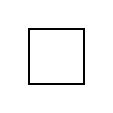
\begin{tikzpicture}[scale=.7]
          \draw[thick](0,0) rectangle(1,1);
        \end{tikzpicture}
      \end{center}
    \end{enumerate}
    \vspace{1in}
    
  \item Suppose that there is a passenger of mass \SI{70}{\kilo\gram} in the
    elevator. Calculate the apparent weight of the passenger at time
    $t=\SI{4}{\second}$.
  \end{enumerate}
  \vspace{1in}
  \newpage
  
  % TAKEN FROM 2001 AP PHYSICS B EXAM FREE-RESPONSE QUESTION 2
  \cpic{.7}{table1}
  
\item An incident ball $A$ of mass \SI{.10}{\kilo\gram} is sliding at
  \SI{1.4}{\metre\per\second} on the horizontal tabletop of negligible friction
  shown above. It makes a head-on collision with a target ball $B$ of mass
  \SI{.50}{\kilo\gram} at rest at the edge of the table. As a result of the
  collision, the incident ball rebounds, sliding backwards at
  \SI{.70}{\metre\per\second} immediately after the collision.
  \begin{enumerate}[nosep]
  \item Calculate the speed of the \SI{.50}{\kilo\gram} target ball immediately
    after the collision.
  \end{enumerate}
  The tabletop is 1.20 m above a level, horizontal floor. The target ball is
  projected horizontally and initially strikes the floor at a horizontal
  displacement $d$ from the point of collision.
  \begin{enumerate}[nosep]
  \item Calculate the horizontal displacement $d$.
  \end{enumerate}
  \newpage
  
  \cpic{.6}{table2}
  In another experiment on the same table, the target ball $B$ is replaced by
  target ball $C$ of mass 0.10 kg. The incident ball $A$ again slides at
  \SI{1.4}{\metre\per\second}, as shown above left, but this time makes a
  glancing collision with the target ball $C$ that is at rest at the edge of
  the table. The target ball $C$ strikes the floor at point $P$, which is at a
  horizontal displacement of \SI{.15}{\metre} from the point of the collision,
  and at a horizontal angle of \ang{30} from the $+x$-axis, as shown above
  right.
  \begin{enumerate}[nosep]
  \item Calculate the speed $v$ of the target ball $C$ immediately after the
    collision.
  \item Calculate the $y$-component of incident ball $A$'s momentum immediately
    after the collision.
  \end{enumerate}
  \newpage


  
  % TAKEN FROM 2016 AP PHYSICS 1 FREE-RESPONSE QUESTION 3
  \begin{center}
    \pic{.8}{ramp-down}\\
    \underline{Note:} Figure not drawn to scale.
  \end{center}
\item (Suggested time 25 minutes) A long track, inclined at an angle $\theta$
  to the horizontal, has small speed bumps on it. The bumps are evenly spaced a
  distance $d$ apart, as shown in the figure above. The track is actually much
  longer than shown, with over 100 bumps. A cart of mass $M$ is released from
  rest at the top of the track. A student notices that after reaching the
  40th bump the cart's average speed between successive bumps no longer
  increases, reaching a maximum value $v_\mathrm{avg}$. This means the time
  interval taken to move from one bump to the next bump becomes constant.
  \begin{enumerate}[nosep]
  \item Consider the cart's motion between bump 41 and bump 44.
    \begin{enumerate}[nosep]
    \item In the figure below, sketch a graph of the cart's velocity $v$ as a
      function of time from the moment it reaches bump 41 until the moment it
      reaches bump 44.
    \item Over the same time interval, draw a dashed horizontal line at
      $v=v_\text{avg}$. Label this line ``$v_\text{avg}$''.
    \end{enumerate}
    \begin{center}
      \begin{tikzpicture}
        \draw[thick,->](0,0)--(4,0) node[pos=0,left]{0} node[pos=1,right]{Time};
        \draw[thick,->](0,0)--(0,3) node[pos=1,above]{$v$};
        \draw[dashed](.2,-.1)--(.2,2.8) node[pos=0,below]{41};
        \draw[dashed](1.2,-.1)--(1.2,2.8) node[pos=0,below]{42};
        \draw[dashed](2.2,-.1)--(2.2,2.8) node[pos=0,below]{43};
        \draw[dashed](3.2,-.1)--(3.2,2.8) node[pos=0,below]{44};
      \end{tikzpicture}
    \end{center}
  \item Suppose the distance between the bumps is increased but everything else
    stays the same. Is the maximum speed of the cart now greater than, less
    than, or the same as it was with the bumps closer together?

    \vspace{.2in}
    \underline{\hspace{.25in}} Greater than\hspace{.5in}
    \underline{\hspace{.25in}} Less than\hspace{.5in}
    \underline{\hspace{.25in}} Same as

    \vspace{.2in}Briefly explain your reasoning.
    \vspace{.4in}
  \item With the bumps returned to the original spacing, the track is tilted to
    a greater ramp angle $\theta$. Is the maximum speed of the cart greater
    than, less than, or the same as it was when the ramp angle was smaller?

    \vspace{.2in}
    \underline{\hspace{.25in}} Greater than\hspace{.5in}
    \underline{\hspace{.25in}} Less than\hspace{.5in}
    \underline{\hspace{.25in}} Same as

    \vspace{.2in}Briefly explain your reasoning.
    \newpage

  \item Before deriving an equation for a quantity such as $v_\text{avg}$, it
    can be useful to come up with an equation that is intuitively expected to
    be true. That way, the derivation can be checked later to see if it makes
    sense physically. A student comes up with the following equation for the
    cart's maximum average speed:\\
    $\displaystyle v_\text{avg}=C\frac{Mg\sin\theta}{d}$, where $C$ is a
    positive constant.
    \begin{enumerate}[nosep]
    \item To test the equation, the student rolls a cart down the long track
      with speed bumps many times in front of a motion detector. The student
      varies the mass $M$ of the cart with each trial but keeps everything else
      the same. The graph shown below is the student's plot of the data for
      $v_\text{avg}$ as a function of $M$.
      \cpic{.4}{results}
      Are these data consistent with the student's equation?

      \vspace{.1in}
      \underline{\hspace{.25in}} Yes\hspace{.5in}
      \underline{\hspace{.25in}} No

      \vspace{.1in}Briefly explain your reasoning.\vspace{.4in}

    \item Another student suggests that whether or not the data above are
      consistent with the equation, the equation could be incorrect for other
      reasons. Does the equation make physical sense?

      \vspace{.1in}
      \underline{\hspace{.25in}} Yes\hspace{.5in}
      \underline{\hspace{.25in}} No
    
      \vspace{.1in}Briefly explain your reasoning.\vspace{1in}
    \end{enumerate}
  \end{enumerate}
  \newpage
  
  % Tipler Chapter 3 Question 72
\item A projectile is launched from point O at an angle of \ang{22} with an
  initial velocity of \SI{15}{\metre\per\second} up an incline plane that makes
  an angle of \ang{10} with the horizontal. The projectile hits the incline
  plane at point M.
  \cpic{.35}{incline}
  \begin{enumerate}[nosep]
  \item Find the time it takes for the projectile to hit the incline plane.
  \item Find the distance OM.
  \end{enumerate}
  \vspace{\stretch{1}}
  
%\item A steel ball is dropped from a point with $(x,y)$ coordinate of
%  $(\SI{8}{\metre},\SI{16}{\metre})$. At the same time, another ball is launched
%  from the origin with a speed of \SI{20}{\metre\per\second} at an angle of
%  \ang{30}.
%  \begin{enumerate}[nosep]
%  \item Find the minimum distance of separation occur of the two balls.
%  \item At what time does this separation occur?
%  \item Give the coordinates of the two balls for the minimum separation.
%  \end{enumerate}

\item A high-powered rifle shoots bullets that leave the mizzle at
  \SI{1.1e3}{\metre\per\second}. If a bullet is to hit a target
  \SI{950}{\metre} away at the level, the gun must be aimed at a point above
  the target. Neglecting air resistance, how far above the target is this
  point?
  \vspace{\stretch{1}}

  
%\item A trail bike take off from a ramp with velocity $\mb{v}_0$ at angle
%  $\theta$ to clear a ditch of width $x$ and land on the other side, which is
%  elevated at a height $H$.
%  \cpic{.4}{trail-bike}
%  \begin{enumerate}[nosep]
%  \item For a given angle $\theta$ and distance $x$, what is the upper limit
%    for $H$ such that the bike has an chance of making the jump?
%  \item For $H$ less than this upper limit, what is the minimum take-off speed
%    $v_0$ necessary for a successful jump?
%  \end{enumerate}
%  Neglect the size of the trail bike, and assume that covering a horizontal
%  distance $x$ and a vertical distance $H$ is sufficient to clear the ditch.
\end{enumerate}
\end{document}
